\documentclass[12pt]{article}
\usepackage{amsmath, amsthm, amssymb}
\usepackage{hyperref}
\usepackage[margin=1cm]{caption}
\usepackage{verbatim}
\usepackage[top=1.0in, bottom=1.0in, left=1.0in, right=1.0in]{geometry}
\usepackage{graphicx}

\pagestyle{plain}

\usepackage{tkz-graph}
\usetikzlibrary{arrows}
\usetikzlibrary{shapes}
\usepackage[position=bottom]{subfig}

\usepackage{longtable}
\usepackage{array}

\usepackage{sectsty}
\allsectionsfont{\sffamily}

\setcounter{secnumdepth}{5}
\setcounter{tocdepth}{5}

\makeatletter
\newtheorem*{rep@theorem}{\rep@title}
\newcommand{\newreptheorem}[2]{
\newenvironment{rep#1}[1]{
 \def\rep@title{#2 \ref{##1}}
 \begin{rep@theorem}}
 {\end{rep@theorem}}}
\makeatother

\theoremstyle{plain}
\newtheorem{thm}{Theorem}[section]
\newreptheorem{thm}{Theorem}
\newtheorem{prop}[thm]{Proposition}
\newreptheorem{prop}{Proposition}
\newtheorem{lem}[thm]{Lemma}
\newreptheorem{lem}{Lemma}
\newtheorem{conjecture}[thm]{Conjecture}
\newreptheorem{conjecture}{Conjecture}
\newtheorem{cor}[thm]{Corollary}
\newreptheorem{cor}{Corollary}
\newtheorem{prob}[thm]{Problem}
\newtheorem{observation}{Observation}
\newtheorem{obs}[observation]{Observation}
\newtheorem*{mainconj}{Main Conjecture}
\newtheorem*{mainthm}{Main Theorem}
\newtheorem*{thmA}{Theorem A}
\newtheorem*{stretching}{Stretching Lemma}
\newtheorem{problem}{Problem}
\newtheorem{clm}{Claim}

\theoremstyle{definition}
\newtheorem{defn}{Definition}
\theoremstyle{remark}
\newtheorem*{remark}{Remark}
\newtheorem{example}{Example}
\newtheorem*{question}{Question}


\newcommand{\fancy}[1]{\mathcal{#1}}
\newcommand{\C}[1]{\fancy{C}_{#1}}
\newcommand{\IN}{\mathbb{N}}
\newcommand{\IR}{\mathbb{R}}
\newcommand{\G}{\fancy{G}}
\newcommand{\CC}{\fancy{C}}
\newcommand{\D}{\fancy{D}}

\newcommand{\inj}{\hookrightarrow}
\newcommand{\surj}{\twoheadrightarrow}

\newcommand{\set}[1]{\left\{ #1 \right\}}
\newcommand{\setb}[3]{\left\{ #1 \in #2 \mid #3 \right\}}
\newcommand{\setbs}[2]{\left\{ #1 \mid #2 \right\}}
\newcommand{\card}[1]{\left|#1\right|}
\newcommand{\size}[1]{\left\Vert#1\right\Vert}
\newcommand{\ceil}[1]{\left\lceil#1\right\rceil}
\newcommand{\floor}[1]{\left\lfloor#1\right\rfloor}
\newcommand{\func}[3]{#1\colon #2 \rightarrow #3}
\newcommand{\funcinj}[3]{#1\colon #2 \inj #3}
\newcommand{\funcsurj}[3]{#1\colon #2 \surj #3}
%\newcommand{\irange}[1]{\left[#1\right]}
\newcommand{\irange}[1]{\left\{1,\ldots,#1\right\}}
\newcommand{\join}[2]{#1 \mbox{\hspace{2 pt}$\ast$\hspace{2 pt}} #2}
\newcommand{\djunion}[2]{#1 \mbox{\hspace{2 pt}$+$\hspace{2 pt}} #2}
\newcommand{\parens}[1]{\left( #1 \right)}
\newcommand{\brackets}[1]{\left[ #1 \right]}
\newcommand{\nint}[1]{\widetilde{N}\left(#1\right)}
\newcommand{\DefinedAs}{\mathrel{\mathop:}=}
\newcommand{\pot}{\operatorname{pot}}

\def\D{\fancy{D}}
\def\C{\fancy{C}}
\def\Q{\fancy{Q}}
\def\Z{\fancy{Z}}
%\def\H{\fancy{H}}
\def\L{\fancy{L}}
\def\B{\fancy{B}}
\def\erdos{Erd\H{o}s}

% any changes to \claim should be mirrored in \claimnonum and \subclaim
\newcommand{\claim}[2]{{\bf Claim #1.}~{\it #2}~~}
\newcommand{\claimnonum}[1]{{\bf Claim.}~{\it #1}~~}
%\newcommand{\subclaim}[2]{{\bf Subclaim #1.}~{\it #2}~~}

%\newcommand\numberthis{\addtocounter{equation}{1}\tag{\theequation}}

%
%  If the proof ends with a displayed equation, use \aftermath just
%  before \end{proof} to put the halmos in the ``right'' place.  This
%  may not work near page boundaries. 
%
\def\aftermath{\par\vspace{-\belowdisplayskip}\vspace{-\parskip}\vspace{-\baselineskip}}

\def\fr{\frac}
\def\adj{\leftrightarrow}
\def\nonadj{\not\!\leftrightarrow}
\def\ch{\textrm{ch}}
\renewcommand{\restriction}{\mathord{\upharpoonright}}

\begin{document}
\title{Beyond Degree Choosability}
\author{Daniel W. Cranston\thanks{Department of Mathematics and Applied
Mathematics, Viriginia Commonwealth University, Richmond, VA;
\texttt{dcranston@vcu.edu}; 
Research of the first author is partially supported by NSA Grant
98230-15-1-0013.}
\and
Landon Rabern\thanks{LBD Data Solutions, Lancaster, PA;
\texttt{landon.rabern@gmail.com}}
}

\maketitle
\begin{abstract}
Let $G$ be a connected graph with maximum degree $\Delta$.  Brooks' theorem
states that $G$ has a $\Delta$-coloring unless $G$ is a complete graph or an
odd cycle.  A graph $G$ is \emph{degree-choosable} if $G$ can be properly
colored from its lists whenever each vertex $v$ gets a list of $d(v)$ colors.
In the context of list coloring, Brooks' theorem can be strengthened to the
following.  Every connected graph $G$ is degree-choosable unless each block of
$G$ is a complete graph or an odd cycle; such a graph $G$ is a \emph{Gallai
tree}.  

This degree-choosability result was further strengthened to Alon--Tarsi orientations;
these are orientations of $G$ in which the numbers of spanning Eulerian
subgraphs with an even number of edges differs from the number with an odd
number of edges.  A graph $G$ is \emph{degree-AT} if $G$ has an Alon--Tarsi
orientation such that each vertex has indegree at least 1.  Hladky, Kral, and
Schauz showed that a connected graph is degree-AT if and only if it is not a
Gallai tree.  In this paper, we consider pairs $(G,x)$ where $G$ is a connected
graph and $x$ is some specified vertex in $V(G)$.  We characterize pairs such
that $G$ has no Alon--Tarsi orientation in which each vertex has indegree at
least 1 and $x$ has indegree at least 2.  When $G$ is 2-connected, the
characterization is simple to state.
\end{abstract}

\section{Introduction}

Brooks' theorem is one of the fundamental results in graph coloring.
For every connected graph $G$, it says that $G$ has a $\Delta$-coloring
unless $G$ is a clique $K_{\Delta+1}$ or an odd cycle.  When we seek to prove coloring
results by induction, we often want to color a subgraph $H$ where different vertices
have different lists of allowable colors (those not already used on their
neighbors in the coloring of $G-H$).  This gives rise to \emph{list coloring}.
Vizing~\cite{vizing1976} and, independently, \erdos, Rubin, and
Taylor~\cite{ERT} extended Brooks'
theorem to list coloring. They proved an analogue of Brooks' theorem
when each vertex $v$ has $\Delta$ allowable colors (possibly
different colors for different vertices).  In fact, they proved the following
strengthening, where a \emph{Gallai tree} is a connected graph in which each
block is a clique or an odd cycle.  

\begin{thmA}
If $G$ is connected and not a Gallai tree, then for any list assignment $L$
with $|L(v)|=d(v)$ for all $v\in V(G)$, graph $G$ has a proper coloring
$\varphi$ with $\varphi(v)\in L(v)$ for all $v$.  
\end{thmA}

The graphs in Theorem~A are \emph{degree-choosable}.  It is easy to check
that every Gallai tree is not degree-choosable.  So the set of all
connected graphs that are not degree-choosable are precisely the Gallai trees.
Hladky, Kral, and Schauz~\cite{HKS} extended this characterization to the setting of
Alon--Tarsi orientations.

For any digraph $D$, a spanning Eulerian subgraph is one in which each vertex
has indegree equal to outdegree.  The \emph{parity} of a spanning Eulerian
subgraph is the parity of its number of edges.  For an orientation of a graph
$G$, let EE (resp.~EO) denote the number of even (resp.~odd) spanning Eulerian
subgraphs.  An orientation is \emph{Alon--Tarsi} (or AT) if EE and
EO differ.  A graph $G$ is $f$-AT if it has an Alon--Tarsi
orientation $D$ such that $d^+(v)\le f(v)-1$ for each vertex $v$.  In
particular, $G$ is \emph{degree-AT} if it is $f$-AT, where $f(v)=d(v)$ for all
$v$.  Alon and Tarsi~\cite{AlonT} used algebraic methods to show that if $G$ is
$f$-AT, for any $f$, then $G$ also has a proper coloring $\varphi$ from any
list assignment $L$ such that $|L(v)|=f(v)$ for all $v\in V(G)$; such a graph
$G$ is \emph{$f$-choosable}.

In this paper we characterize those graphs $G$ with a specified vertex $x$
that are not $f$-AT, where $f(x)=d(x)-1$ and $f(v)=d(v)$ for all other $v\in
V(G)$.  All such graphs are formed from a few 2-connected building blocks, by
repeatedly applying two operations.  Similar to that for degree-AT, our
characterization remains unchanged in the contexts of list-coloring and
paintability.  We see a sharp contrast when we consider graphs $G$ with two
specified vertices $x_1$ and $x_2$ that are not $f$-AT, where
$f(x_i)=d(x_i)-1$ for each $i\in \{1,2\}$ and $f(v)=d(v)$ for all other
$v\in V(G)$.  For Alon--Tarsi orientations, we have more than 50 exceptional
graphs on seven vertices or fewer.  Furthermore, the characterizations for
list-coloring, paintability, and Alon--Tarsi orientations all differ.

\bigskip

We consider graphs with vertices labeled by natural numbers; that is, pairs
$(G,h)$ where $G$ is a graph and $\func{h}{V(G)}{\IN}$.  We focus on the case
when $h(x)=1$ for some $x$ and $h(v)=0$ for all other $v$; we denote this
labeling as $h_x$.  We say that \emph{$(G, h)$ is AT} if $G$ is $(d_G - h)$-AT.
 When $H$ is an induced subgraph of $G$, we simplify notation by referring to
the pair $(H, h)$ when we really mean $\parens{H, h\restriction_{V(H)}}$.

Given a pair $(G,h)$ and a specified edge $e\in E(G)$, when we \emph{stretch
$e$}, we form $(G',h')$ from $(G,h)$ by subdividing $e$ twice and
setting $h'(v_i)=0$ for each of the two new vertices, $v_1$ and $v_2$ (and
$h'(v)=h(v)$ for all other vertices $v$).  
In Section~\ref{prelims}, we prove
a \hyperref[SubdivideTwice]{Stretching Lemma}, which shows that if $(G,h)$ is not AT and $e\in E(G)$, then
stretching $e$ often yields another pair $(G',h')$ that is also not AT. 
Thus, stretching plays a key role in our main result.

It is easy to check that the three pairs $(G,h)$ shown in Figure~1 are not AT.
Let $\D$ be the collection of all pairs formed from the graphs in Figure~1 by
stretching each bold edge 0 or more times.  The
\hyperref[SubdivideTwice]{Stretching Lemma} implies that
each pair in $\D$ is not AT.  Our main result is that these are the only
pairs $(G,h_x)$, where $G$ is 2-connected and neither a clique nor an
odd cycle, such that the $(G,h_x)$ is not AT (for some vertex $x\in V(G)$).  

\begin{mainthm}
Let $G$ be 2-connected and let $x \in V(G)$.
Now $(G,h_x)$ is AT if and only if
\begin{enumerate}
\item $d(x)=2$ and $G-x$ is not a Gallai tree; or
\item $d(x)\ge 3$, $G$ is not complete, and $(G,h_x) \not \in \D$.
\end{enumerate}
\end{mainthm}

Near the end of Section~\ref{MainThmSec}, with a little more work we extend our
Main Theorem, by removing the hypothesis of 2-connectedness, to characterize
all pairs $(G,h_x)$ that are not AT.
The characterization of degree-choosable graphs have been applied
to prove a variety of graph coloring
results~\cite{BohmeMS, CranstonPTV, KostochkaS, KralS, Thomassen-surface}. 
Likewise, we think our main results in this paper may be helpful in proving
other results for Alon--Tarsi orientations, such as giving better lower bounds
on the number of edges in AT-critical graphs.

%\begin{comment}
\begin{figure}[htb]
	\centering
	\tikzstyle{_BoldEdgeStyle} = [line width=3]
	\begin{tikzpicture}[scale = 10]
	\tikzstyle{VertexStyle} = []
	\tikzstyle{EdgeStyle} = []
	\tikzstyle{labeledStyle}=[shape = circle, minimum size = 6pt, inner sep = 1.2pt, draw]
	\tikzstyle{unlabeledStyle}=[shape = circle, minimum size = 6pt, inner sep = 1.2pt, draw, fill]
	\Vertex[style = labeledStyle, x = 0.800, y = 0.850, L = \small {$1$}]{v0}
	\Vertex[style = labeledStyle, x = 0.700, y = 0.700, L = \small {$0$}]{v1}
	\Vertex[style = labeledStyle, x = 0.900, y = 0.700, L = \small {$0$}]{v2}
	\Vertex[style = labeledStyle, x = 0.800, y = 0.550, L = \small {$0$}]{v3}
	\Edge[style = _BoldEdgeStyle, label = \small {}, labelstyle={auto=right, fill=none}](v1)(v0)
	\Edge[style = _BoldEdgeStyle, label = \small {}, labelstyle={auto=right, fill=none}](v2)(v0)
	\Edge[style = _BoldEdgeStyle, label = \small {}, labelstyle={auto=right, fill=none}](v3)(v0)
	\Edge[label = \small {}, labelstyle={auto=right, fill=none}](v1)(v2)
	\Edge[label = \small {}, labelstyle={auto=right, fill=none}](v3)(v2)
	\Edge[label = \small {}, labelstyle={auto=right, fill=none}](v1)(v3)
	\end{tikzpicture}\hspace{.3in}
	\begin{tikzpicture}[scale = 10]
	\tikzstyle{VertexStyle} = []
	\tikzstyle{EdgeStyle} = []
	\tikzstyle{labeledStyle}=[shape = circle, minimum size = 6pt, inner sep = 1.2pt, draw]
	\tikzstyle{unlabeledStyle}=[shape = circle, minimum size = 6pt, inner sep = 1.2pt, draw, fill]
	\Vertex[style = labeledStyle, x = 1.300, y = 0.450, L = \small {$0$}]{v0}
	\Vertex[style = labeledStyle, x = 1.200, y = 0.300, L = \small {$0$}]{v1}
	\Vertex[style = labeledStyle, x = 1.400, y = 0.300, L = \small {$0$}]{v2}
	\Vertex[style = labeledStyle, x = 1.050, y = 0.300, L = \small {$0$}]{v3}
	\Vertex[style = labeledStyle, x = 1.550, y = 0.300, L = \small {$0$}]{v4}
	\Vertex[style = labeledStyle, x = 1.300, y = 0.600, L = \small {$0$}]{v5}
	\Vertex[style = labeledStyle, x = 1.300, y = 0.750, L = \small {$1$}]{v6}
	\Edge[label = \small {}, labelstyle={auto=right, fill=none}](v1)(v0)
	\Edge[label = \small {}, labelstyle={auto=right, fill=none}](v1)(v2)
	\Edge[label = \small {}, labelstyle={auto=right, fill=none}](v2)(v0)
	\Edge[style = _BoldEdgeStyle, label = \small {}, labelstyle={auto=right, fill=none}](v3)(v1)
	\Edge[style = _BoldEdgeStyle, label = \small {}, labelstyle={auto=right, fill=none}](v4)(v2)
	\Edge[style = _BoldEdgeStyle, label = \small {}, labelstyle={auto=right, fill=none}](v5)(v0)
	\Edge[style = _BoldEdgeStyle, label = \small {}, labelstyle={auto=right, fill=none}](v6)(v3)
	\Edge[style = _BoldEdgeStyle, label = \small {}, labelstyle={auto=right, fill=none}](v6)(v4)
	\Edge[style = _BoldEdgeStyle, label = \small {}, labelstyle={auto=right, fill=none}](v6)(v5)
	\end{tikzpicture}\hspace{.3in}
	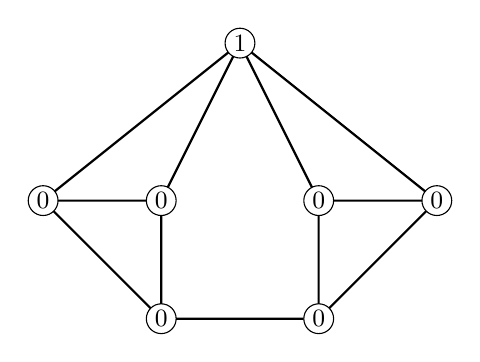
\begin{tikzpicture}[scale = 10]
	\tikzstyle{VertexStyle} = []
	\tikzstyle{EdgeStyle} = []
	\tikzstyle{labeledStyle}=[shape = circle, minimum size = 6pt, inner sep = 1.2pt, draw]
	\tikzstyle{unlabeledStyle}=[shape = circle, minimum size = 6pt, inner sep = 1.2pt, draw, fill]
	\Vertex[style = labeledStyle, x = 1.000, y = 0.250, L = \small {$0$}]{v0}
	\Vertex[style = labeledStyle, x = 1.200, y = 0.250, L = \small {$0$}]{v1}
	\Vertex[style = labeledStyle, x = 0.850, y = 0.400, L = \small {$0$}]{v2}
	\Vertex[style = labeledStyle, x = 1.000, y = 0.400, L = \small {$0$}]{v3}
	\Vertex[style = labeledStyle, x = 1.350, y = 0.400, L = \small {$0$}]{v4}
	\Vertex[style = labeledStyle, x = 1.200, y = 0.400, L = \small {$0$}]{v5}
	\Vertex[style = labeledStyle, x = 1.100, y = 0.600, L = \small {$1$}]{v6}
	\Edge[label = \small {}, labelstyle={auto=right, fill=none}](v0)(v2)
	\Edge[label = \small {}, labelstyle={auto=right, fill=none}](v0)(v3)
	\Edge[label = \small {}, labelstyle={auto=right, fill=none}](v1)(v0)
	\Edge[label = \small {}, labelstyle={auto=right, fill=none}](v2)(v3)
	\Edge[label = \small {}, labelstyle={auto=right, fill=none}](v4)(v1)
	\Edge[label = \small {}, labelstyle={auto=right, fill=none}](v5)(v1)
	\Edge[label = \small {}, labelstyle={auto=right, fill=none}](v5)(v4)
	\Edge[label = \small {}, labelstyle={auto=right, fill=none}](v6)(v2)
	\Edge[label = \small {}, labelstyle={auto=right, fill=none}](v6)(v3)
	\Edge[label = \small {}, labelstyle={auto=right, fill=none}](v6)(v4)
	\Edge[label = \small {}, labelstyle={auto=right, fill=none}](v6)(v5)
	\end{tikzpicture}
	\caption{The seed blocks for $\D$.  Each bold edge can be removed without
making the figure AT.}
	\label{fig:seeds}
\end{figure}
%\end{comment}

%We conclude with a few definitions.  When vertices $x$ and $y$ are adjacent, we
%write $x\adj y$; otherwise, $x\nonadj y$.
%[Define paintability and AT.]

\section{Subgraphs, subdivisions, and cuts}
\label{prelims}

When Hladky, Kral, and Schauz characterized degree-AT graphs, their proof relied
heavily on the observation that a connected graph $G$ is degree-AT if and only
if $G$ has some induced subgraph $H$ such that $H$ is degree-AT.  Below, we
reprove this easy lemma, and also extend it to our setting of pairs $(G,h_x)$.


\begin{lem}\label{InducedSubgraph}
Let $G$ be a connected graph and let $H$ be an induced subgraph of $G$.  If $H$
is degree-AT, then
also $G$ is degree-AT.  
Similarly, if $x\in V(H)$ and $(H,h_x)$ is AT, then also $(G,h_x)$ is AT.
Further, if $x\notin V(H)$ and $d_G(x)\ge 2$, then $(G,h_x)$ is AT.  
\end{lem}
\begin{proof}
Suppose that $H$ is degree-AT, and let $D'$ be an orientation of $H$ showing
this.  Extend $D'$ to an orientation $D$ of $G$ by orienting all edges away from
$H$, breaking ties arbitrarily, but consistently.  Now every directed cycle in
$D$ is also a directed cycle in $D'$ (and vice versa), so $G$ is degree-AT.
The proof of the second statement is identical.  The proof of the third
statement is similar, but now if some edge $xy$ has endpoints equidistant from
$H$, then $xy$ should be oriented into $x$.
\end{proof}

Recall that, given a pair $(G,h)$ and a specified edge $e\in E(G)$, when we
\emph{stretch $e$}, we form $(G',h')$ from $(G,h)$ by subdividing $e$ twice
and setting $h'(v_i)=0$ for each of the two new vertices, $v_1$ and $v_2$
(and $h'(v)=h(v)$ for all other vertices $v$).  By repeatedly stretching edges,
starting from the pairs in Figure~1, we form all pairs $(G,h_x)$, where $G$ is
2-connected and $(G,h_x)$ is not AT.  

\begin{stretching}\label{SubdivideTwice}
Form $(G',h')$ from $(G,h)$ by stretching some edge $e\in E(G)$.
%subdividing an edge $e$ of $G$ twice and
%setting $h'(v_i)=0$ for each of the two new vertices, $v_1$ and $v_2$. 
Now
\begin{enumerate}
\item[(1)] if $(G,h)$ is AT, then $(G', h')$ is AT; and
\item[(2)] if $(G', h')$ is AT, then either $(G,h)$ is AT or $(G-e,h)$ is AT.
\end{enumerate}	
\end{stretching}
\begin{proof}
Suppose $e = u_1u_2$ and call the new vertices $v_1$ and $v_2$ so that $G'$ contains
the induced path $u_1v_1v_2u_2$.  For (1), let $D$ be an orientation of $G$ showing
that $(G,h)$ is AT. By symmetry we may assume $u_1u_2 \in E(D)$. Form an
orientation $D'$ of $G'$ from $D$ by replacing $u_1u_2$ with the directed path
$u_1v_1v_2u_2$.  We have a natural parity preserving bijection between the spanning
Eulerian subgraphs of $D$ and $D'$, so we conclude that $(G', h')$ is AT.
	
For (2), let $D'$ be an orientation of $G'$ showing that $(G',h')$ is AT. 
Suppose $G'$ contains the directed path $u_1v_1v_2u_2$ or the directed path
$u_2v_2v_1u_1$.
 By symmetry, we can assume it is $u_1v_1v_2u_2$.  Now form an orientation $D$ of
$G$ by replacing $u_1v_1v_2u_2$ with the directed edge $u_1u_2$.  As above, we have a
parity preserving bijection between the spanning Eulerian subgraphs of $D$ and
$D'$, so we conclude that $(G, h)$ is AT.  Otherwise, no spanning Eulerian
subgraph of $D'$ contains a cycle passing through $v_1$ and $v_2$.  So, the
spanning Eulerian subgraph counts of $D'$ are the same as those of $D' - v_1 -
v_2$.  However, this gives an orientation of $G-e$ showing that $(G-e, h)$ is AT.
\end{proof}

Given a pair $(G,h)$ that is not AT, the \hyperref{SubdivideTwice}[Stretching
Lemma] suggests a way to
construct a larger graph $G'$ such that $(G',h')$ is not AT.  Specifically, we
have the following.
\begin{cor}\label{SubdivideConstructor}
If $e$ is an edge in $G$ such that $(G,h)$ is not AT and $(G-e, h)$ is not AT,
then stretching $e$ gives a pair $(G',h')$ that is not AT.
%$(G',h')$ is not AT where $(G',h')$ is formed from $(G,h)$ by stretching
%$e$.
%subdividing $e$ twice and having $h'$ give zero on the two new vertices.
\end{cor}

In some cases, we can also use the \hyperref[SubdivideTwice]{Stretching Lemma} to construct a smaller graph
$\widehat{G}$ such that $(\widehat{G},h)$ is not AT.
\begin{cor}\label{ReduceP4Cor}
Let $G$ be a graph with an induced path $u_1v_1v_2u_2$ such that $d_G(v_1) =
d_G(v_2) = 2$.  If $(G,h)$ is AT, where $h(v_1) = h(v_2) = 0$, and
$(G-v_1-v_2,h)$ is not AT, then \[\parens{(G - v_1 - v_2) + u_1u_2,
h\restriction_{V(G) \setminus \set{v_1, v_2}}} \text{ is AT.}\]
\end{cor}
\begin{proof}
Suppose the pair $(G,h)$ satisfies the hypotheses.
Applying part (2) of the \hyperref[SubdivideTwice]{Stretching Lemma} shows that either $\parens{G - v_1
- v_2, h\restriction_{V(G) \setminus \set{v_1, v_2}}}$ is AT or $\parens{(G -
v_1 - v_2) + u_1u_2, h\restriction_{V(G) \setminus \set{v_1, v_2}}}$ is AT. 
By hypothesis, the former is false.  Thus, the latter is true.
%But $G - x_2 - x_3$ is a proper induced subgraph of $G$, so the former cannot
%happen since $G$ is $h$-greedy-minimal and $h(x_2) = h(x_3) = 0$.  Hence
%$\parens{(G - x_2 - x_3) + x_1x_4, h\restriction_{V(G) \setminus \set{x_2,
%x_3}}}$ is AT.
\end{proof}

With standard vertex coloring, we can easily reduce to the case where $G$ is
2-connected.  If $G$ is a connected graph with two blocks, $B_1$ and $B_2$,
meeting at a cutvertex $x$, then we can color each of $B_1$ and $B_2$
independently, and afterward we can permute colorings to match at $x$.
For Alon--Tarsi orientations, the situation is not quite as simple.  However,
the following lemma plays a similar role for us.

\begin{lem}\label{CutvertexPatch}
Let $A_1, A_2 \subseteq V(G)$, and $x\in V(G)$ be such that $A_1\cup A_2=V(G)$ and $A_1 \cap
A_2 = \set{x}$.  If $G[A_i]$ is $f_i$-AT for each $i \in \{1,2\}$, then $G$ is
$f$-AT, where $f(v) = f_i(v)$ for each $v \in V(A_i-x)$ and $f(x) = f_1(x) + f_2(x)
- 1$.  Going the other direction, if $G$ is $f$-AT, then $G[A_i]$ is $f_i$-AT
for each $i \in \{1,2\}$, where $f_i(v) = f(v)$ for each $v \in V(A_i-x)$ and
$f_1(x) + f_2(x) \le f(x) + 1$.
\end{lem}
\begin{proof}
We begin with the first statement.
For each $i \in \{1,2\}$, choose an orientation $D_i$ of $A_i$ showing that $A_i$
is $f_i$-AT.  Together these $D_i$ give an orientation $D$ of $G$. Since no cycle
has vertices in both $A_1-x$ and $A_2-x$, we have
\begin{align*}
EE(D) - EO(D) &= EE(D_1)EE(D_2) + EO(D_1)EO(D_2) - EE(D_1)EO(D_2) - EO(D_1)EE(D_2) \\
&= (EE(D_1) - EO(D_1))(EE(D_2) - EO(D_2)) \\
&\ne 0.
\end{align*}
Hence $G$ is $f$-AT.
	
Now we prove the second statement.  Suppose that $G$ is $f$-AT and choose an
orientation $D$ of $G$ showing this. 
Let $D_i = D[A_i]$ for each $i \in \{1,2\}$.  As above, we have $0 \ne
EE(D) - EO(D) = (EE(D_1) - EO(D_1))(EE(D_2) - EO(D_2))$. Hence, $EE(D_1) -
EO(D_1) \ne 0$ and $EE(D_2) - EO(D_2) \ne 0$.  Since the indegree of $x$ in
$D$ is the sum of the indegree of $x$ in $D_1$ and the indegree of $x$ in
$D_2$, the lemma follows.
\end{proof}

\section{Degree-AT graphs and an Extension Lemma}
%A graph $G$ is called \emph{degree-AT} if $(G,h)$ is $AT$ where $h(v)=0$ for all
%$v\in V(G)$.
Recall that our Main Theorem relies on a characterization of degree-AT graphs. 
As we mentioned in the introduction, a description of degree-choosable graphs
was first given by Vizing~\cite{vizing1976} and \erdos, Rubin, and
Taylor~\cite{ERT}.  Hladky, Kral, and Schauz~\cite{HKS} later extended the
proof from~\cite{ERT} to Alon--Tarsi orientations.  This proof relies on
Rubin's Block lemma, which states that every 2-connected graph $G$ contains an
induced even cycle with at most one chord, unless $G$ is a clique or an odd
cycle.  For variety, and completeness, we include a new proof; it extends ideas
of Kostochka, Stiebitz, and Wirth~\cite{KSW} from list-coloring to Alon--Tarsi
orientations.  For this proof we need the following very special case of a key
lemma in \cite{OreVizing}.  When vertices $x$ and $y$ are adjacent, we write
$x\adj y$; otherwise $x\nonadj y$.

\begin{lem}\label{GeneralEulerLemma}
Let $G$ be a graph and $x \in V(G)$ such that $H$ is connected, where $H \DefinedAs G-x$. 
If there exist $z_1, z_2 \in V(H)$ with $N_H[z_1] = N_H[z_2]$ such that $x \adj
z_1$ and $x \nonadj z_2$, then $G$ is $f$-AT where $f(x) = 2$ and $f(v) =
d_G(v)$ for all $v \in V(H)$.
\end{lem}
\begin{proof}
Order the vertices of $H$ with $z_1$ first and $z_2$ second so that every
vertex, other than $z_1$, has at least one neighbor preceding it. 
Orient each edge of $H$ from its earlier endpoint toward its later endpoint. 
Orient $xz_1$ into $z_1$ and orient all other
edges incident to $x$ into $x$.  Let $D$ be the resulting orientation. 
Clearly, $d_{D}^+(v) \le f(v) - 1$ for all $v \in V(D)$.  So, we just need to
check that $EE(D) \ne EO(D)$.  

Since $xz_1$ is the only edge of $D$ leaving
$x$, and $D-x$ is acyclic, every spanning Eulerian subgraph of $D$ that has
edges must have edge $xz_1$.  
%
Consider an Eulerian subgraph $A$ of $D$ containing $xz_1$. Since $z_1$ %must
has indegree $1$ in $A$, it must also have outdegree $1$ in $A$.  We show
that $A$ has a mate $A'$ of opposite parity.  
%
If $z_2 \in A$ then $z_1z_2w \in A$, for some $w$, so we form
$A'$ from $A$ by removing $z_1z_2w$ and adding $z_1w$. 
If instead $z_1z_2\notin A$, then $z_2 \not \in A$ and $z_1w \in
A$ for some $w \in N_H[z_1]-z_2$, so we form $A'$ from $A$ by removing $z_1w$ and
adding $z_1z_2w$.  
%
Hence exactly half of the Eulerian subgraphs of $D$ that contain edges are
even.  Since the edgeless spanning subgraph of $D$ is an even Eulerian
subgraph, we conclude that $EE(D) = EO(D) + 1$.  Hence $G$ is $f$-AT.
\end{proof}

We use the previous lemma to give a new proof of the characterization of
degree-AT graphs.
\begin{lem}
\label{DegreeATClassification}
A connected graph $G$ is degree-AT if it is not a Gallai tree.
\end{lem}
\begin{proof}
Suppose there exists a connected graph that is not a Gallai tree, but is also not
degree-AT.  Let $G$ be such a graph with as few vertices as possible.
Since $G$ is not degree-AT, no induced subgraph $H$ of $G$ is
degree-AT by Lemma \ref{InducedSubgraph}. 
Hence, for any $v \in V(G)$ that is not a cutvertex, $G-v$ must be a Gallai
tree by minimality of $|G|$.  
	
If $G$ has more than one block, then for endblocks $B_1$ and $B_2$, choose
noncutvertices $w\in B_1$ and $x\in B_2$.  By the minimality of $|G|$, both
$G-w$ and $G-x$ are Gallai trees.  Since every block of $G$ appears either as a
block of $G-w$ or as a block of $G-x$, every block of $G$ is either complete or
an odd cycle.  Hence, $G$ is a Gallai tree, a contradiction.  So instead $G$
has only one block, that is, $G$ is $2$-connected.  Further, $G-v$ is a Gallai
tree for all $v \in V(G)$.
	
Let $v$ be a vertex of minimum degree in $G$.  Since $G$ is $2$-connected,
$d_G(v) \ge 2$ and $v$ is adjacent to a noncutvertex in every endblock of $G-v$.
If $G-v$ has a complete block $B$ with noncutvertices $x_1,x_2$ where $v \adj
x_1$ and $v \nonadj x_2$, then we can apply Lemma \ref{GeneralEulerLemma} 
%with $Y = \set{v}$ and $F = vx_1$ 
to conclude that $G$ is degree-AT, a
contradiction.  So, $v$ must be adjacent to every noncutvertex in every
complete endblock of $G-v$.
	
Suppose $d_G(v) \ge 3$.  Now no endblock of $G-v$ can be an odd cycle of
length at least $5$ ($G$ would have vertices of degree $3$ and also $d_G(v) \ge
4$, contradicting the minimality of $d_G(v)$).  Let $B$ be a smallest complete
endblock of $G-v$.  Now for a noncutvertex $x \in V(B)$, we have $d_G(x) =
|B|$ and hence $d_G(v) \le |B|$. 
If $G-v$ has at least two endblocks, then $2(|B|-1) \le |B|$, so $d_G(v)
\le |B| = 2$, a contradiction.  Hence, $G-v = B$ and $v$ is joined to $B$, so
$G$ is complete, which is a contradiction.
	
Thus, we have $d_G(v) = 2$.  Suppose $G-v$ has at least two endblocks. 
Now it has exactly two and $v$ is adjacent to one noncutvertex in each. 
Neither of the endblocks can be odd cycles of length at least five, since then
we can get a smaller counterexample by the \hyperref[SubdivideTwice]{Stretching
Lemma}.  Since $v$ is adjacent to every noncutvertex in every
complete endblock of $G-v$, both endblocks must be $K_2$.  But now either
$G=C_4$ (which is trivially degree-AT) or we can get a smaller counterexample
by the \hyperref[SubdivideTwice]{Stretching Lemma}.  So, $G-v$ must be
$2$-connected. Since $G-v$ is a Gallai tree, it is either complete or an odd
cycle.  If $G-v$ is not complete, then we can get a smaller counterexample by
the \hyperref[SubdivideTwice]{Stretching Lemma}.  So, $G-v$ is complete and
$v$ is adjacent to every
noncutvertex of $G-v$; that is, $G$ is complete, a contradiction.
\end{proof}

\section{When h is 1 for at most one vertex}
\label{MainThmSec}
For a graph $G$ and $x \in V(G)$ recall that $\func{h_x}{V(G)}{\IN}$ is defined
as $h_x(x) = 1$ and $h_x(v) = 0$ for all $v \in V(G-x)$. We classify the
connected 
graphs $G$ such that $(G,h_x)$ is AT for some $x \in V(G)$. 
%To start, we reduce to the case when $G$ is $2$-connected.
We begin with the case when $G$ is 2-connected, which takes most of the work.
At the end of the section, we extend this to all connected graphs.

We will show that for most 2-connected graphs $G$ and vertices $x\in V(G)$, the
pair $(G,h_x)$ is AT.  Specifically, this is true for all pairs except those in
$\D$, defined in the introduction.  In view of Lemma~\ref{InducedSubgraph}, for
a 2-connected graph $G$ and $x\in V(G)$, to show $(G,h_x)$ is AT it suffices to
find some induced subgraph $H$, with $x\in V(H)$, such that $(H,h_x)$ is AT. 
The subgraphs $H$ that we consider all have $d_H(x)\ge 3$.  This motivates the
next lemma, which allows us to reduce to the case $d_G(x)\ge 3$.

\begin{lem}\label{DegreeTwoVertex}
If $G$ is a connected graph and $x \in V(G)$ with $d_G(x) = 2$, then $(G,h_x)$
is AT if and only if $G-x$ is degree-AT.
\end{lem}
\begin{proof}
Let $D$ be an orientation of $G$ showing that $(G,h_x)$ is AT.  Then
$d_{D}^-(x) = 2$ and hence no spanning Eulerian subgraph contains a cycle
passing through $x$.  Therefore, the Eulerian subgraph counts in $G-x$ are
different and $G-x$ is degree-AT.  The other direction is immediate from Lemma
\ref{InducedSubgraph}.
\end{proof}
%Let $\D$ be the smallest collection of pairs $(G,h)$ containing the pairs in
%Figure \ref{fig:seeds} that is closed under stretching bold edges.  Explicitly,
%$\D$ is all graphs that can be created from the graphs in Figure
%\ref{fig:seeds} by replacing each bold edge with an odd length path.  The
%rightmost graph in Figure \ref{fig:seeds}  (the Moser Spindle) has no bold edges.

A \emph{$\theta$-graph}, $\Theta_{a,b,c}$, consists of two 3-vertices joined by
three internally disjoint paths, with lengths $a$, $b$, and $c$.  We will see
shortly that if $H$ is a $\theta$-graph with $d_H(x)=3$, then $(H,h_x)$ is AT.
Thus, we can assume that $G$ has no induced $\theta$-graph $H$ with $d_H(x)=3$. 
All of the other
forbidden subgraphs $H$ that we consider (and show that $(H,h_x)$ is AT) can be
viewed as $\theta$-graphs with at most three extra edges.  We show if $G$ is
2-connected with $x\in V(G)$ and $d(x)\ge 3$, then either (i) $G\in \D$ or (ii)
$G$ contains one of these forbidden ``nearly $\theta$-' graphs.

\begin{lem}\label{ThetaReducible}
If $H$ is a $\theta$-graph, $\Theta_{a,b,c}$, with $d_H(x)=3$, then $(H,h_x)$ is AT
(regardless of $a$, $b$, and $c$).
\end{lem}
\begin{proof}
By the \hyperref[SubdivideTwice]{Stretching Lemma}, this follows directly from
the fact that the four pairs
shown in Figure~2 are AT.
\end{proof}

The simplest of our nearly $\theta$-graphs are called $T$ graphs (they have a
single extra edge).  For positive integers $a$, $b$, and $c$, let $T_{a, b, c}$
be the graph consisting of
(i) a triangle $z_1z_2z_3$ and 
(ii) disjoint paths $z_iP_iw_i$ where $P_i$ has length $a_i$ for $i \in \{1,2,3\}$ and
(iii) a vertex $x$ adjacent to $w_1, w_2, w_3$.

\begin{lem}\label{TgraphReducible}
$(T_{a, b, c}, h_x)$ is AT whenever exactly one or two of $a, b$, and
$c$ is even.
\end{lem}
\begin{proof}
By the \hyperref[SubdivideTwice]{Stretching Lemma}, this follows from the fact that Figure
\ref{fig:SubdividedK4} and Figure \ref{fig:TriangleRuinsPath} are AT.
\end{proof}

The graph we consider next can be viewed as a $\theta$-graph, with the three extra
edges among $z_1$, $z_2$, and $z_3$.
\begin{lem}\label{T+graphReducible}
Form $H$ from $T_{a, b, c}$ by adding a new vertex with
neighborhood $\set{z_1, z_2, z_3}$.  Now $(H, h_x)$ is AT.
\end{lem}
\begin{proof}
This follows from Lemma \ref{TgraphReducible} and Lemma
\ref{InducedSubgraph} using Lemma \ref{SubdivideTwice} and the fact that Figure
\ref{fig:K5minus} is AT and Figure \ref{fig:thebigone} is AT.
\end{proof}


\begin{lem}\label{AddPathReducible}
Let $G$ be a $T$-graph. Let $P$ be a path of $G$ where all internal
vertices of $P$ have degree 2 in $G$ and one endvertex of $P$ has degree 2 in
$G$.  Form $G'$ from $G$ by adding a path $P'$ (of length at least 2) joining
the endvertices of $P$.  Now $(G', h_x)$ is AT.
\end{lem}
\begin{proof}
We can assume that $G$ is not AT; otherwise, we are done by Lemma 2.1.
By symmetry, assume $P$ is a subpath $P_3$. First, we get an orientation of $G$
with indegree at least 1 for all vertices and $d^-(x) = 2$. Orient $P_1$
from $z_1$ to $x$, $P_2$ from $z_2$ to $x$, $P_3$ from $x$ to $z_3$, and the triangle
as $z_3z_2$, $z_3z_1$, $z_1z_2$.  To get an orientation of $G'$, orient the
new path $P'$ consistently, and opposite of $P$.  Now the only
directed cycle containing edges of $P'$ is $P'P$.  Since the Eulerian subgraph
counts are equal for $G$, they differ by 1 for $G'$. 
\end{proof}

%\begin{lem}\label{MoserLem}
%If there exists a proper induced subgraph $H$ of $G$ such that $d_H(x)=4$ and $H$ is the Moser
%spindle, shown in Figure~1c, then $(G,h_x)$ is AT.
%\end{lem}
\tikzstyle{majorStyle}=[shape = circle, minimum size = 6pt, inner sep = 2.2pt, draw]
\tikzstyle{major}=[shape = circle, minimum size = 6pt, inner sep = 2.2pt, draw]
\tikzstyle{minorStyle}=[shape = rectangle, minimum size = 6pt, inner sep = 2.2pt, draw]
\tikzstyle{minor}=[shape = rectangle, minimum size = 6pt, inner sep = 2.2pt, draw]
\tikzstyle{labeledStyle}=[shape = rectangle, minimum size = 6pt, inner sep = 2.2pt, draw]
\tikzstyle{VertexStyle} = []
\tikzstyle{EdgeStyle} = []
%\tikzstyle{unlabeledStyle}=[shape = circle, minimum size = 6pt, inner sep = 1.2pt, draw, fill]
\begin{figure}[htb]
\begin{center}
\subfloat[]{\makebox[.33\textwidth]{
\begin{tikzpicture}[scale = 6]
\Vertex[style = major, x = 0.45, y = 0.95, L = \small {$4$}]{v0}
\Vertex[style = major, x = 0.15, y = 0.75, L = \small {$3$}]{v1}
\Vertex[style = major, x = 0.35, y = 0.75, L = \small {$3$}]{v2}
\Vertex[style = major, x = 0.55, y = 0.75, L = \small {$4$}]{v3}
\Vertex[style = major, x = 0.55, y = 0.55, L = \small {$3$}]{v4}
\Edge[label= \small {$e$}, , labelstyle={auto=right, fill=none}](v0)(v1)
\Edge[](v2)(v0)
\Edge[](v2)(v3)
\Edge[](v3)(v0)
\Edge[](v4)(v3)
\draw[white] (0,.475)--(0,0.49);
\end{tikzpicture}
}}
%\subfloat[Figure 2]{\makebox[.5\textwidth]{
%\begin{tikzpicture}[scale = 8]
%\Vertex[style = major, x = 0.400, y = 0.900, L = \small {$u$}]{v0}
%\Vertex[style = minor, x = 0.150, y = 0.700, L = \small {$v_1$}]{v1}
%\Vertex[style = minor, x = 0.300, y = 0.700, L = \small {$v_2$}]{v2}
%\Vertex[style = major, x = 0.500, y = 0.700, L = \small {$v_3$}]{v3}
%\Vertex[style = major, x = 0.650, y = 0.700, L = \small {$v_4$}]{v4}
%\Vertex[style = minor, x = 0.650, y = 0.550, L = \small {$w$}]{v5}
%\Edge[](v1)(v0)
%\Edge[](v2)(v0)
%\Edge[](v2)(v3)
%\Edge[](v3)(v0)
%\Edge[](v4)(v0)
%\Edge[](v5)(v4)
%\end{tikzpicture}
%}}
\subfloat[]{\makebox[.33\textwidth]{
\begin{tikzpicture}[scale = 7]
%\begin{scope}[xshift=.7cm,yshift=.1cm]
\Vertex[style = major, x = 0.5, y = 0.849, L = \small {$4$}]{v0}
\Vertex[style = major, x = 0.200, y = 0.650, L = \small {$3$}]{v1}
\Vertex[style = major, x = 0.400, y = 0.650, L = \small {$3$}]{v2}
\Vertex[style = major, x = 0.600, y = 0.650, L = \small {$4$}]{v3}
\Vertex[style = major, x = 0.800, y = 0.650, L = \small {$4$}]{v4}
\Vertex[style = major, x = 0.550, y = 0.449, L = \small {$3$}]{v6}
\Vertex[style = major, x = 0.649, y = 0.449, L = \small {$3$}]{v5}
\Vertex[style = major, x = 0.800, y = 0.449, L = \small {$3$}]{v7}
\Edge[label= \small {$e$}, , labelstyle={auto=right, fill=none}](v0)(v1)
\Edge[](v2)(v0)
\Edge[](v3)(v0)
\Edge[](v4)(v0)
\Edge[](v5)(v3)
\Edge[](v6)(v3)
\Edge[](v7)(v4)
\end{tikzpicture}
}}
%\end{scope}
%}}
%
%\subfloat[]{\makebox[.5\textwidth]{
%\begin{tikzpicture}[scale = 8]
%\Vertex[style = major, x = 0.500, y = 0.849, L = \small {$u$}]{v0}
%\Vertex[style = minor, x = 0.400, y = 0.650, L = \small {$v_1$}]{v2}
%\Vertex[style = minor, x = 0.500, y = 0.650, L = \small {$v_2$}]{v1}
%\Vertex[style = major, x = 0.600, y = 0.650, L = \small {$v_3$}]{v3}
%\Vertex[style = major, x = 0.800, y = 0.650, L = \small {$v_4$}]{v4}
%\Vertex[style = minor, x = 0.500, y = 0.449, L = \small {$w_1$}]{v6}
%\Vertex[style = minor, x = 0.699, y = 0.449, L = \small {$w_2$}]{v5}
%\Edge[label= \small {$e$}, , labelstyle={auto=right, fill=none}](v0)(v2)
%\Edge[](v1)(v0)
%\Edge[](v3)(v0)
%\Edge[](v4)(v0)
%\Edge[](v4)(v5)
%\Edge[](v5)(v3)
%\Edge[](v6)(v3)
%\end{tikzpicture}
%}}
\subfloat[]{\makebox[.33\textwidth]{
\begin{tikzpicture}[rotate=90,scale=7]
%\begin{tikzpicture}[yshift=.253cm,xshift=2.8cm,rotate=90,scale=7]
\Vertex[style = major, x = 0.35, y = 0.80, L = \small {$3$}]{v0}
\Vertex[style = major, x = 0.65, y = 0.80, L = \small {$3$}]{v1}
\Vertex[style = major, x = 0.50, y = 0.65, L = \small {$4$}]{v2}
\Vertex[style = major, x = 0.50, y = 0.95, L = \small {$4$}]{v3}
\Vertex[style = major, x = 0.50, y = 0.50, L = \small {$4$}]{v4}
\Vertex[style = major, x = 0.50, y = 0.35, L = \small {$3$}]{v5}
\Edge[](v2)(v0)
\Edge[label= \small {$e$}, , labelstyle={auto=right, fill=none}](v2)(v1)
\Edge[](v3)(v0)
\Edge[](v3)(v1)
\Edge[](v4)(v2)
\Edge[](v5)(v4)
\draw[white] (.26,.55)--(.27,.55);
\end{tikzpicture}
}}
%\end{scope}
\end{center}
\caption{Each configuration is reducible by deleting edge $e$.
(The number at each vertex specifies its degree in G.)\label{fig:hiltonzhao}}
\end{figure}
%Vertices drawn as circles have degree 4 in $G$ and vertices drawn as rectangles
%have degree 3 in $G$.  


%\newpage
%\clearpage
%\pagebreak

\begin{lem}\label{TwoConnectedClassification}
Let $G$ be 2-connected, and choose $x\in V(G)$ with $d(x)\ge 3$. 
Now $(G,h_x)$ is AT if and only if $G$ is not complete and $(G,h_x) \not \in \D$.
\end{lem}
\begin{proof}
	First suppose that $(G,h_x)\in \D$.  Add details.
	
	Now let $G$ be 2-connected, choose $x\in V(G)$ with $d(x)\ge 3$, and suppose that
	$(G,h_x)\notin \D$.
	Since $G-x$ is connected, let $H'$ be a smallest connected
	subgraph of $G-x$ containing three neighbors of $x$; call these neighbors
	$w$, $y$, and $z$.  
	Consider a spanning tree $T$ of $H'$.  Since $H'$ is minimum, each leaf of $T$
	is among $\{w, y, z\}$.  If $T$ is a path, then $H'$ is also a path. 
	Otherwise, $T$ is a subdivision of $K_{1,3}$.  Let $s$ be the vertex with
	$d_T(s)=3$.  If $E(G)-E(T)$ has any edge with
	both ends outside of $N(s)$, then we can delete some vertex in $N(s)$ and remain
	connected, contradicting the minimality of $H'$.  Similarly, if $N(s)$ contains
	at least two edges, then $H'-s$ still connects, $w$, $y$, and $z$.  Now let $H$
	be the subgraph of $G$ induced by $V(H')\cup\{x\}$.  Note that $H$ is either
	a $\theta$-graph (if $H'$ is a tree) or a $T$-graph (if $H'$ has one extra edge in
	$N(s)$).  
	
	If $H$ is a $\theta$-graph, then $(G,h_x)$ is AT, by
	Lemma~\ref{ThetaReducible} and Lemma~\ref{InducedSubgraph}.
	So assume $H$ is a $T$-graph.  Let $z_1$, $z_2$, $z_3$ be the vertices
	of degree 3 (other than $x$), and let $P_1$, $P_2$, and $P_3$ denote the paths
	from $x$ to $z_1$, $z_2$, and $z_3$; when we write $V(P_i)$, we exclude $x$ and
	$z_i$, so possibly $V(P_i)$ is empty for one or more $i\in\{1,2,3\}$.
	If any two of $P_1$, $P_2$, and $P_3$ have lengths with opposite parities, then
	we are done by Lemma~\ref{TgraphReducible}; so assume not.  
	
	Now $(H,h_x)\in \D$, so we can assume that $V(G-H) \ne \emptyset$.  
	For $u \in V(G-H)$, let $H_u$ be a minimal $2$-connected induced subgraph of $G$ that contains $V(H) \cup \set{u}$.  
	Since $G-x$ is a Gallai tree, so is $H_u-x$; in particular, the block $B_u$ of $H_u-x$ containing $u$ is complete or an odd cycle.  
	Therefore, we either have (i) $V(B_u) \cap V(H) = \set{z_1, z_2,z_3}$ or (ii)  $V(B_u) \cap V(H) \subseteq P_i \cup \set{z_i}$ for some $i \in \irange{3}$.
	
	Suppose (i) happens. Then $N_G(u) \cap V(H_u - x) = \set{z_1,z_2,z_3}$. If $x \nonadj u$, then $(G,h_x)$ is AT by Lemma~\ref{InducedSubgraph} and Lemma~\ref{T+graphReducible}.
	If $x \adj u$, then $x \adj z_i$ for all $i \in \irange{3}$ since otherwise $(G,h_x)$ is AT by Lemma~\ref{InducedSubgraph} and Lemma~\ref{T+graphReducible}.  So, $H=K_4$ and $H_u$ is $K_5$.  
	This implies that (ii) cannot happen for any vertex in $V(G-H)$. So (i) happens for every vertex in $V(G-H)$; in particular, $V(G-H)$ is joined to $\set{x,z_1,z_2,z_3}$.  Since $G$ is not complete, it must contain an induced Figure \ref{fig:K5minus} and hence $(G,h_x)$ is AT by Lemma~\ref{InducedSubgraph}.
		
	So, we may assume that (ii) happens for every vertex in $V(G-H)$. Pick $u \in V(G - H)$. By symmetry, we may assume that $V(B_u) \cap V(H) \subseteq P_1$.
	Say $P_1 = v_1v_2\cdots v_{\ell}$ where $v_1 = z_1$ and $v_{\ell}$ is adjacent to $x$.	First, assume $B_u$ is an odd cycle of length at least $5$.  If there is $u' \in V(B_u)\setminus V(H)$ with $u' \adj x$, then $G$ contains a $\theta$-graph and  $(G,h_x)$ is AT, by	Lemma~\ref{ThetaReducible} and Lemma~\ref{InducedSubgraph}.  So, we may assume that $u' \nonadj x$ for all $u' \in V(B_u)\setminus V(H)$.  If $B_u$ contains at least two edges of $H$, then we can replace $P_1$ with a path of the opposite parity (by going around the cycle) and we are done by Lemma~\ref{TgraphReducible}.  But, if $B_u$ contains only one edge of $H$, then $H$ is a stretching of Figure~\ref{fig:WingedCows} or Figure~\ref{fig:thebiggerones}.
	
	So, we may assume that $B_u$ is complete. Then $V(B_u) \cap V(H) = \set{v_{j}, v_{j+1}}$ for some $j \in \irange{\ell}$.  
	In particular, $B_u$ is a triangle.  If $j \ne \ell - 1$, then $(G,h_x)$ is AT by Lemma~\ref{InducedSubgraph} and Figure~\ref{fig:thebiggerones}. 	By Lemma \ref{GeneralEulerLemma}, $(G,h_x)$ is AT unless $x \adj u$.  
	So, $H_u$ is a $T$-graph with a vertex $u$ added that is adjacent to $x$ and a $K_2$ endblock $D_u$ of $H-x$.  If $u_1, u_2$ are different vertices in $V(G-H)$ such that $D_{u_1} = D_{u_2}$, then $G$ contains an induced Figure \ref{fig:K5minus} and hence $(G,h_x)$ is AT by Lemma~\ref{InducedSubgraph}. Say $H-x$ has $t \le 3$ endblocks that are $K_2$. Then we must have $|V(G - H)| \le t$.   If $t = 0$, then $G = H$ is the Moser spindle.  If $t=1$, then $G = H_u$ is the Moser spindle for the one $u \in V(G-H)$.  So, we may assume that $t \in \set{2,3}$.    But now $G$ contains an induced stretching of a graph in Figure~\ref{fig:WingedCows}.
	
%	Suppose $u_1, u_2$ are different vertices in $V(G-H)$.  Say $V(D_{u_i}) = \set{x_i, y_i}$ for $i \in \irange{2}$ where $x_i \adj x$.  If $y_1 \nonadj y_2$, then $G$ has an induced subgraph containing consisting of two diamonds sharing $x$.  But then  %$(G,h_x)$ is AT by Lemma~\ref{CutvertexPatch} and Lemma~\ref{InducedSubgraph}.  So, $y_1\adj y_2$.  But now $G$ contains an induced Figure~\ref{fig:WingedCows}(a).  Hence, we must have $|V(G - H)| = 1$. 
\end{proof}

%\begin{proof}
%First suppose that $(G,h_x)\in \D$.  Add details.
%
%Now let $G$ be 2-connected, choose $x\in V(G)$ with $d(x)\ge 3$, and suppose that
%$(G,h_x)\notin \D$.
%Since $G-x$ is connected, let $H'$ be a smallest connected
%subgraph of $G-x$ containing three neighbors of $x$; call these neighbors
%$w$, $y$, and $z$.  
%Consider a spanning tree $T$ of $H'$.  Since $H'$ is minimum, each leaf of $T$
%is among $\{w, y, z\}$.  If $T$ is a path, then $H'$ is also a path. 
%Otherwise, $T$ is a subdivision of $K_{1,3}$.  Let $s$ be the vertex with
%$d_T(s)=3$.  If $E(G)-E(T)$ has any edge with
%both ends outside of $N(s)$, then we can delete some vertex in $N(s)$ and remain
%connected, contradicting the minimality of $H'$.  Similarly, if $N(s)$ contains
%at least two edges, then $H'-s$ still connects, $w$, $y$, and $z$.  Now let $H$
%be the subgraph of $G$ induced by $V(H')\cup\{x\}$.  Note that $H$ is either
%a $\theta$-graph (if $H'$ is a tree) or a $T$-graph (if $H'$ has one extra edge in
%$N(s)$).  
%
%If $H$ is a $\theta$-graph, then $(G,h_x)$ is AT, by
%Lemma~\ref{ThetaReducible} and Lemma~\ref{InducedSubgraph}.
%So assume $H$ is a $T$-graph.  Let $z_1$, $z_2$, $z_3$ be the vertices
%of degree 3 (other than $x$), and let $P_1$, $P_2$, and $P_3$ denote the paths
%from $x$ to $z_1$, $z_2$, and $z_3$; when we write $V(P_i)$, we exclude $x$ and
%$z_i$, so possibly $V(P_i)$ is empty for one or more $i\in\{1,2,3\}$.
%If any two of $P_1$, $P_2$, and $P_3$ have lengths with opposite parities, then
%we are done by Lemma~\ref{TgraphReducible}; so assume not.  
%
%Now $(H,h_x)\in \D$, so we can assume there exists $u\in V(G-H)$. 
%Since $G$ is 2-connected, consider how $u$ can attach to $H$.  In particular,
%$u$ must have have at least two disjoint paths (possibly single edges), $P_4$ and $P_5$,
%to $H$.  Choose $u$ to minimize the sum of the lengths of $P_4$ and $P_5$. 
%%among such $u$, choose one with the fewest neighbors in $H$.  
%We consider the following cases.
%%First, suppose that $u\nonadj x$ and neither path ends at $x$.  
%%Suppose further that $P_4$ and $P_5$ end on the
%%same path $P_i$ (for some $i\in \{1,2,3\}$).  By minimality of $H'$, $u$ has at
%%most three edges to $P_i$.  More precisely, all neighbors of $u$ on $P_i$ are within
%%distance at most two of each other.  If $u$ has at most two neighbors on $P_i$,
%%then we are done by Claim~1.  Otherwise, $u$ has exactly three neighbors on
%%$P_i$.  Together, these four vertices induce $K_4-e$, which is degree-AT.
%%Now we are done by Lemma~\ref{InducedSubgraph}.  So suppose instead that $P_4$
%%and $P_5$ end on different paths, say on $P_2$ and $P_3$.
%%Now $G-x$ again contains a theta graph ($z_2$ and $z_3$ are the two vertices of
%%degree 3); thus, we are done by Lemma~\ref{InducedSubgraph}.
%%
%%Now we assume instead that for every $u\in V(G-H)$, either $u\adj x$ or else at
%%most one path from $u$ to $H$ ends somewhere other than $x$.  Choose $u$ to
%%minimize the sum of the lengths of $P_4$ and $P_5$.  We can assume that $u$ has
%%at least three neighbors in $H$, since otherwise, we are done by Claim~1.  In
%%particular, $u\adj x$.
%
%%\item 
%First suppose $|N_H(u)|\le 2$.
%Consider the subgraph induced by $H$, $u$, and the vertices of $P_4$ and $P_5$.
%First suppose that $P_4$ and $P_5$ both end at vertices in $\{x,z_1,z_2,z_3\}$.
%If one of these endpoints is $x$, then we have a $\theta$-graph $J$ with
%$d_J(x)=3$, so we are done by Lemma~\ref{ThetaReducible} and
%Lemma~\ref{InducedSubgraph}.  If neither path ends at $x$, then we have a
%$\theta$-
%subgraph $J$ with $x\notin J$, so we are again done by the same two lemmas.
%Otherwise, at least one of $P_4$ and $P_5$ ends at a vertex of degree 2 in $H$.
%Now we are done by Lemma~\ref{AddPathReducible}.
%
%%\item 
%%\begin{enumerate}
%Instead assume $|N_H(u)|\ge 3$.  First suppose that $u\nonadj x$.
%Suppose further that $\{z_1,z_2,z_3\}\subseteq N_H(u)$.  If $u$ has only these three
%neighbors, then we are done by Figure~3 or Figure~7 (and the stretching lemma).
%So suppose $u$ has another neighbor, $w$. Choose such a $w$ as close as possible
%to $z_1, z_2, z_3$; by symmetry, say that $w$ is on $P_1$.
%Now $H-x$ has a $\theta$-graph induced by $u, w, z_1, z_2$, and the portion of
%$P_1$ from $w$ to $z_1$.  Thus, we conclude that  $\{z_1,z_2,z_3\}\not\subseteq N_H(u)$.
%If $u$ has exactly two neighbors in $\{z_1,z_2,z_3\}$, then $u, z_1, z_2, z_3$
%induces $K_4-e$, which is a $\theta$-graph;  so assume not.
%Suppose $u$ has neighbors in
%$V(P_i)\cup \{z_i\}$ for at least two $i\in\{1,2,3\}$, say $i=1$ and $i=2$; by
%symmetry, we can assume that $u\nonadj z_3$. 
%Consider the graph induced by $u, z_1, z_2, z_3$, and the paths from the
%neighbor of $u$ on $P_1$ nearest to $z_1$ and the neighbor of $u$ on $P_2$
%nearest to $z_2$.  This subgraph is a $\theta$-graph.  Thus, there must exist some
%$i$ such that $N_H(u)\subseteq z_i\cup V(P_i)$.  Since $d_H(u)\ge 3$, $H-x$
%contains a $\theta$-graph, so we are done.  
%
%Instead, assume that $u\adj x$.
%First suppose that $u$ has a neighbor in $V(P_1)\cup \{z_1\}$
%and $u$ also has a neighbor in $V(P_2)$.  Let $w_1$ be the neighbor of $u$
%nearest to $x$ along $P_1$ and let $w_2$ be the neighbor of $u$ nearest to $x$
%along $P_2$.  Consider the subgraph $J$ induced by $x$, $u$, $w_1$, $w_2$, and the
%paths along $P_1$ and $P_2$ from $x$ to $w_1$ and $w_2$.  Since $J$ is a
%$\theta$-
%graph with $d_J(x)=3$, we are done.  So $u$ must not have neighbors in these two
%sets.  Thus, by symmetry, we can assume either (i) $N(u)\subseteq
%V(P_1)\cup\{z_1\}$ or (ii) $N(u)\subseteq \{x,z_1,z_2,z_3\}$.
%
%Suppose we are in case (i).
%Since $d_H(u)\ge 3$ (and by the minimality of $H'$, and thus $H$), 
%vertex $u$ is adjacent to precisely $x$ and the first two vertices along $P_1$
%(one of which is possibly $z_1$).  
%If $P_1$ or $P_2$ has vertices, then let $J$ be the subgraph induced by $u$ and
%$V(H)\setminus V(P_3)$.  Note that $J-z_3$ is a $\theta$-graph, so $J$ is reducible
%by Lemma~\ref{AddPathReducible}.  Thus, we assume that $V(P_2)=V(P_3)=\emptyset$.
%This implies that $u$ is not adjacent to $z_1$,
%since all $V(P_i)$ have the same parity, by Lemma~\ref{TgraphReducible}.  
%So $|V(P_1)|$ is even.  If $|V(P_1)|\ge 4$, then consider the subgraph $J$ induced
%by $\{u\}\cup N_H(u)\cup (V(H)\setminus V(P_1))$.  Note that $J$ has two blocks
%and $x$ is its cutvertex.  Since neither block is a clique or an odd cycle,
%$(J,h_x)$ is AT by Lemma~\ref{CutvertexPatch}.  Thus, we conclude that
%$|V(P_1)|=2$, so $H$ is the Moser Spindle, shown in Figure~1c.  Since
%$(H,h_x)\in\D$, we can assume that $H\subsetneq G$.  However, now we are done by
%Lemma~\ref{MoserLem}.
%
%Suppose instead that we are in case (ii).  First, suppose there exists $z_i$
%such that $u\nonadj z_i$.  Now $u,z_1,z_2,z_3$ induce a $\theta$-graph in $H-x$, so
%we are done by Lemmas~\ref{ThetaReducible} and \ref{InducedSubgraph}.  Thus, we
%assume that $N_H(u)=\{x,z_1,z_2,z_3\}$.  Let $J$ be a maximum clique containing
%$x$.  We can assume that $G$ is not complete, so there exists some vertex $w$
%outside of $J$.  Since $G$ is 2-connected, $w$ has two vertex disjoint paths to
%$J$, not both ending at the same vertex; let $J'$ denote the subgraph induced
%by $x$, $J$, and the vertices of these two paths.  If neither path ends at $x$,
%then $J'-x$ is 2-connected and not a clique or an odd cycle.  Now
%Lemmas~\ref{DegreeATClassification} and \ref{InducedSubgraph} imply that $(G,h_x)$
%is AT.
%
%Suppose instead that one path from $w$ to $J$ ends at $x$; by symmetry, assume
%the other ends at $z_1$.  Since $w\notin V(J)$, vertex $w$ has some non-neighbor
%in $J$; by symmetry, say it is $z_2$.  Now let $J''$ be the subgraph induced by
%$x, z_1, z_2, w$, and the paths from $w$ to $x$ and $z_1$.  Note that $J''$ is a
%$\theta$-graph with $d_{J''}(x)=3$, so Lemmas~\ref{ThetaReducible} and
%\ref{InducedSubgraph} imply that $(G,h_x)$ is AT.
%\end{proof}


\begin{thm}
If $G$ is connected and $x \in V(G)$, then $(G, h_x)$ is not AT if and only if
\end{thm}

\begin{enumerate}
\item[(1)] $d(x) = 1$; or
\item[(2)] $G$ is a Gallai tree; or
\item[(3)] $d(x) = 2$ and $G-x$ has a component that is a Gallai tree; or
\item[(4)] $x$ is a cutvertex, all but at most one $x$-lobe of G is a Gallai
tree and for every $x$-lobe $H$ of $G$, we have $(G, h_x)$ is not AT; or
\item[(5)] $x$ is not a cutvertex and for the block $B$ of $G$ containing $x$,
we have $(B,h_x) \in \D$ and all $B$-lobes of $G$ are Gallai trees.
\end{enumerate}

\begin{proof}
First, lets check that if any of (1)--(5) happen, then $(G, h_x)$ is not AT.  1 and 2
are immediate.  3 follows from Lemma 4.2. 4 follows from Lemma 2.2. 5 follows
from Lemma 4.9 and Lemma 2.2.

Now, for the other direction, suppose $(G, h_x)$ is not AT and none of
(1)--(5) happen.  By Lemma 4.2 (and not 1 and not 3) we must have $d(x) \ge 3$. 
Suppose $x$ is a cutvertex.  Then (by not 4), at least two $x$-lobes of $G$ are
not Gallai trees or $(H, h_x)$ is AT for some $x$-lobe $H$ of $G$.  But then
$(G,h_x)$ is AT by Lemma 2.2, a contradiction.  So, $x$ is not a cutvertex. 
Suppose the block $B$ of $G$ containing $x$ is complete or $(B,h_x) \in \D$. 
Now (by not 2 and not 5) some $B$-lobe $H$ of $G$ is not a Gallai tree.  Since
$G-x$ is connected, we conclude that $G-x$ is degree-AT and by directing all
edges incident to $x$ into $x$, we get that $(G,h_x)$ is AT, a contradiction. 
By Lemma 2.2, we know that $(B, h_x)$ is not AT. Since B is 2-connected, the
argument in the Lemma in the last email
shows that B is \textbf{$h_x$-minimal}.  We just learned that $B$ is not
complete and $(B,h_x) \not \in \D$, so applying Lemma 4.9 shows that $(B, h_x)$
is AT, a contradiction.
\end{proof}

%\begin{defn}
%A graph $G$ is \emph{$h$-minimal} if $G$ is connected and $\parens{H, h}$ is
%not AT for every proper induced subgraph $H$ of $G$.  A graph $G$ is
%\emph{$h$-greedy-minimal} if $G$ is connected and $\parens{H, h}$ is not AT for
%every proper induced subgraph $H$ of $G$ where $h(v) = 0$ for all $v \in V(G)
%\setminus V(H)$. Note that if $G$ is $h$-minimal then it is also $h$-greedy-minimal.
%\end{defn}
%
%\begin{lem}\label{TwoConnectedReduction}
%	Let $G$ be $h_x$-minimal for $x \in V(G)$ and let $\B$ be the set of
%blocks of $G$ containing $x$.  Now $(G,h_x)$ is AT if and only if
%	\begin{enumerate}
%		\item $\B$ contains at least two degree-AT graphs; or
%		\item $G$ is $2$-connected and $(G, h_x)$ is AT.
%	\end{enumerate}
%\end{lem}
%\begin{proof}
%	Since $G$ is $h_x$-minimal, no block outside of $\B$ is degree-AT.  The lemma
%follows since if $G$ is not $2$-connected, then $(G,h_x)$ is AT if and only if
%(1) holds by Lemma \ref{CutvertexPatch}.
%\end{proof}

\section{Choosability and Paintability}
As we mentioned in the introduction, Alon and Tarsi showed that if a graph $G$
is $f$-AT, then $G$ is also $f$-choosable.  \emph{Online list coloring}, also
called \emph{painting} is similar to list coloring, but now the list for each
vertex is progressively revealed, as the graph is colored. 
Schauz~\cite{schauz2010flexible} extended the Alon--Tarsi theorem, to show that
if $G$ is $f$-AT, then $G$ is also $f$-paintable.  In this section, we use our
characterization of pairs $(G,h_x)$ that are not AT to prove characterizations
of pairs $(G,h_x)$ that are not paintable and that are not choosable.  More
precisely, a pair $(G,h_x)$ is \emph{choosable} if $G$ has a proper coloring
from its lists $L$ whenever $L$ is such that $|L(x)|=d(x)-1$ and $|L(v)|=d(v)$
for all other $v$; otherwise $(G,h_x)$ is \emph{not choosable}.  The definition
of a pair being paintable is analogous.  We characterizes all pairs $(G,h_x)$,
where $G$ is connected and $(G,h_x)$ is not choosable (resp. paintable).  We
will see that, in fact, these characterizations (for both choosability and
paintability) are identical to that for pairs that are not AT.  

Since all pairs $(G,h_x)$ that are AT are also both paintable and choosable, it
suffices to show that every pair $(G,h_x)$ that is not AT is also not choosable
(here we use that if a pair is paintable, then it is also choosable).

\begin{thm}
For every connected graph $G$, the pair $(G,h_x)$ is not choosable if and only
if $(G,h_x)$ is not AT.  Thus, the same characterization holds for pairs that
are not paintable.
\end{thm}

Also, show that when we move up to two vertices $x,y$ with $h(x) =
h(y) = 1$, AT, choosability and paintability all
separate.

\section{Applications}
When this is in a critical graph, we get $h_x$-minimality for free.  If $x$ has
$t \ge 5$ neighbors in one component of the low vertex subgraph, then those
neighbors are all in one $K_t$ block.  If $t = 4$, then the neighbors are
either a $K_4$ block or we create the Moser
Spindle.

\bibliographystyle{abbrv}
\bibliography{GraphColoring1}

\end{document}
